%!TEX program = xelatex
\documentclass[10pt,a4paper,UTF8]{article}
\usepackage{ctex}
\usepackage{indentfirst,latexsym,bm,amsmath,amsthm,enumerate,graphicx,setspace,subfigure,cite,fancyhdr,float}
\usepackage[vmargin=2.54cm,hmargin=3.18cm]{geometry}
%\setmainfont{DengXian}
%\setCJKmainfont{DengXian}

\begin{document}
%~~~~~~~~~~~~~~~~~~~~~~~~~~~~~~~修正部分~~~~~~~~~~~~~~~~~~~~~~~~~~~~~~~~~~~~~~~~~~~~~~~~~~
    %通用修正
    \setlength{\parindent}{2em}                        %首行缩进2字符
    \renewcommand{\baselinestretch}{1.5}\normalsize    %修改行距为标准的x倍

    %中文相关的修正
    \renewcommand*{\qedsymbol}{[证毕]}                 %中文的证x明毕
    \newcommand{\HEI}{\CJKfamily{hei}}                 %中文黑体
    \newcommand{\KAI}{\CJKfamily{kai}}                 %中文楷体

    %英文修正
    \newcommand{\romannum}[1]{\expandafter{\romannumeral#1}}    %罗马字符

    %添加新的定理环境
    \newtheorem{instance}{\HEI例}[section]

    %~~~~~~~~~~~~~~~~~~~~~~~~~~~~~~~修正结束~~~~~~~~~~~~~~~~~~~~~~~~~~~~~~~~~~~~~~~~~~~~~~~~
    \begin{titlepage}
        \title{Venique的SmartGit小课堂\footnote{Made By \LaTeX}}
        \author{Venique}


        \maketitle
        \thispagestyle{empty}
        
        \vspace{0.55\textheight}
        
        \rightline{Venique}
        \rightline{venique@live.com}
    \end{titlepage}

    \newpage

    \pagestyle{fancy}
    \chead{SmartGit设置教程}
    \lhead{Venique}
    \rfoot{\thepage} 
    \cfoot{}
    \section{更新}
        (数据删除):

            由于Venique的粗心,实际设置SmartGit的流程与本教程略有不符。请自行寻找对应的界面在本教程中的位置

        5/12/2016更新:

            由于服务器弱口令被黑客攻破,因此修改git仓库密码,并禁用了git账户登录权限

            密码修改为asdfvbnm

    \section{SmartGit安装}
        到 http://www.syntevo.com/smartgit/download 下载对应版本即可

        下载安装时一路默认设置即可
        \begin{figure}[H]
            \centering
            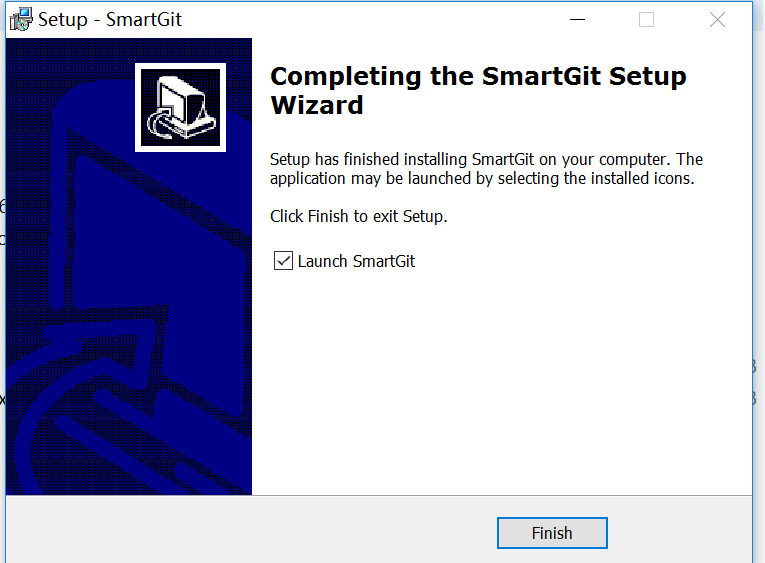
\includegraphics[width=0.8\textwidth]{installed.PNG}
            \caption{安装完成}
        \end{figure}

    \newpage

    \section{SmartGit初始设置}
        下面进行打开SmartGit后的初始设置:
        \begin{figure}[H]
            \centering
            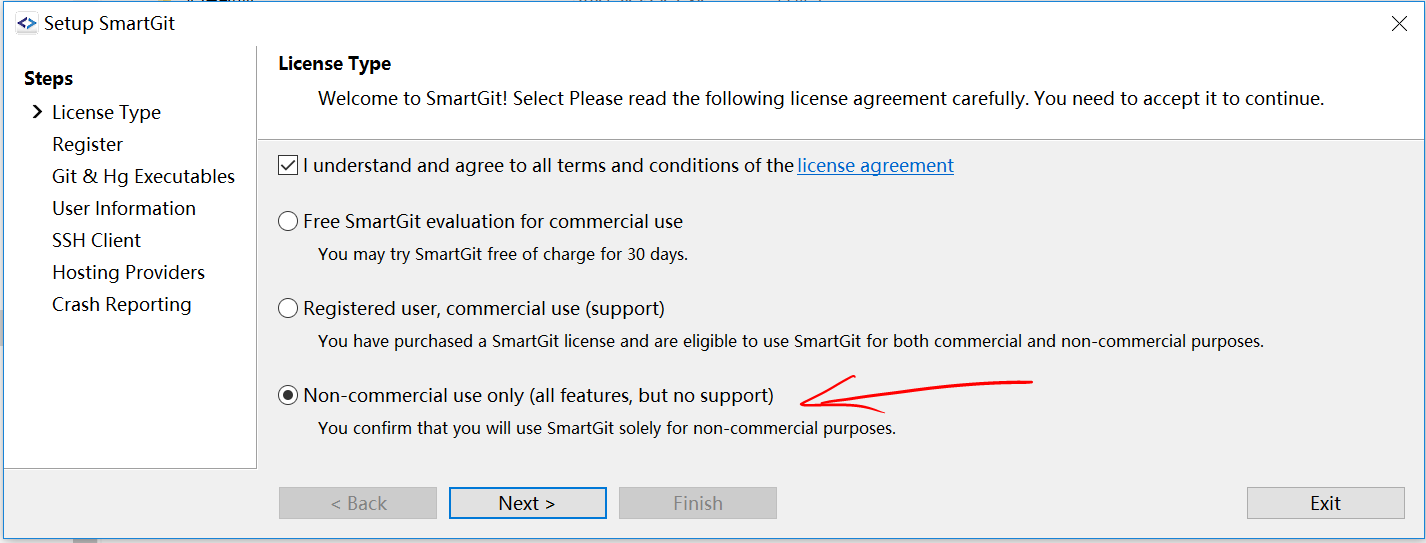
\includegraphics[width=0.8\textwidth]{non-commercial.PNG}
            \caption{选择非商业许可}
        \end{figure}

        \begin{figure}[H]
            \centering
            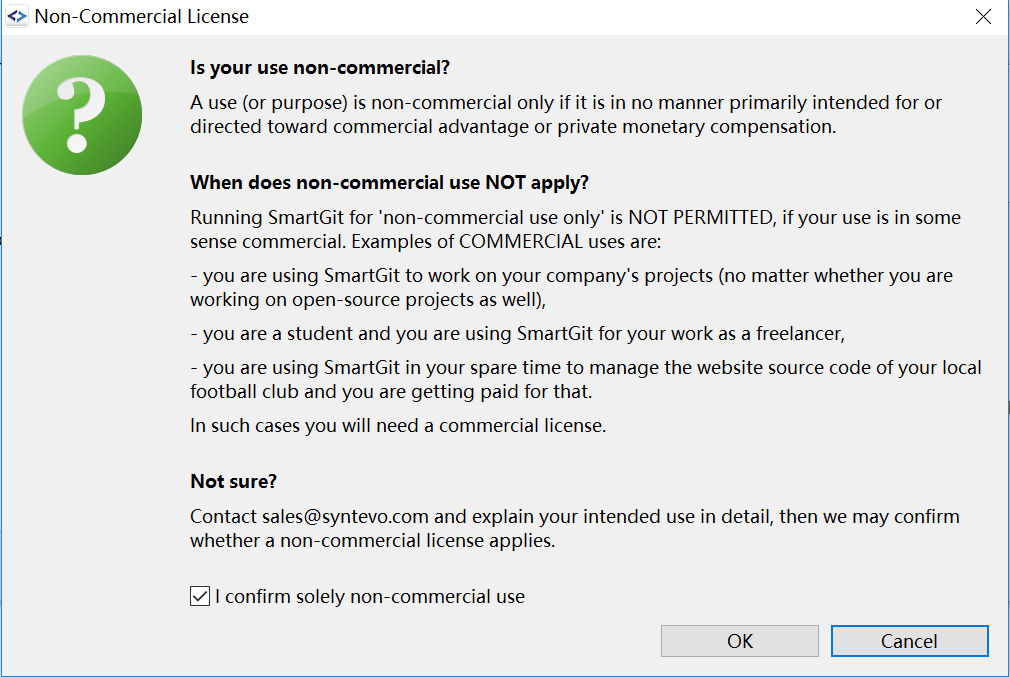
\includegraphics[width=0.8\textwidth]{confirm.PNG}
            \caption{确认非商业许可通知}
        \end{figure}

        \begin{figure}[H]
            \centering
            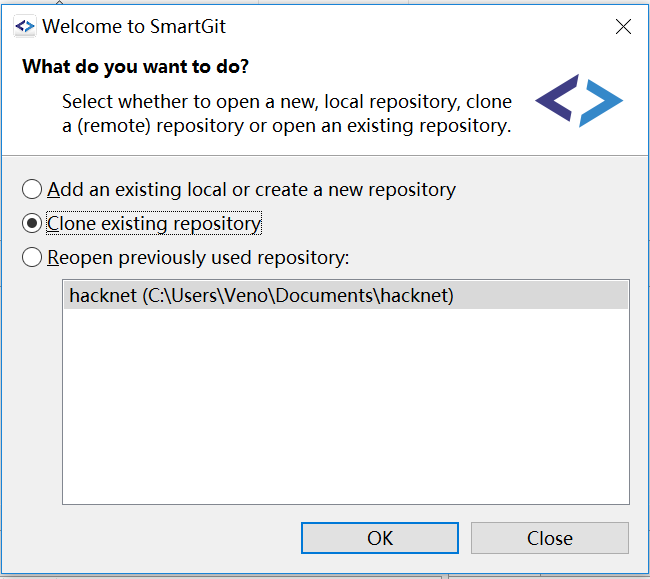
\includegraphics[width=0.8\textwidth]{clone-confirm.PNG}
            \caption{选择克隆已有的git仓库}
        \end{figure}

        最重要的一步:设置远程git仓库路径:如图\ref{fig:setting}

        路径: ssh://git@115.28.12.194/home/git/hacknet.git

        密码: 123456

        \begin{figure}[H]
            \centering
            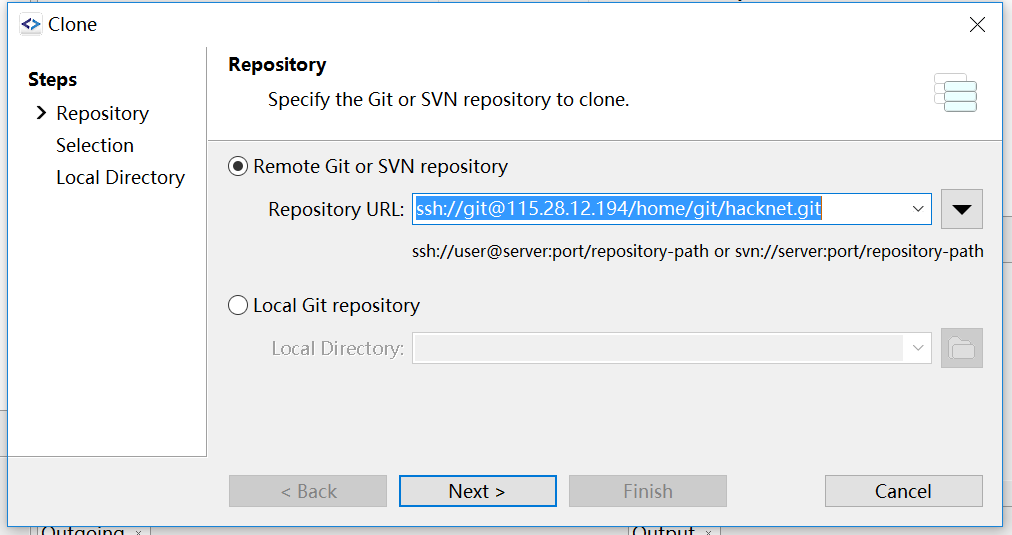
\includegraphics[width=0.8\textwidth]{setting.PNG}
            \caption{设置git仓库路径,请照图片填写}
            \label{fig:setting}
        \end{figure}        

        \begin{figure}[H]
            \centering
            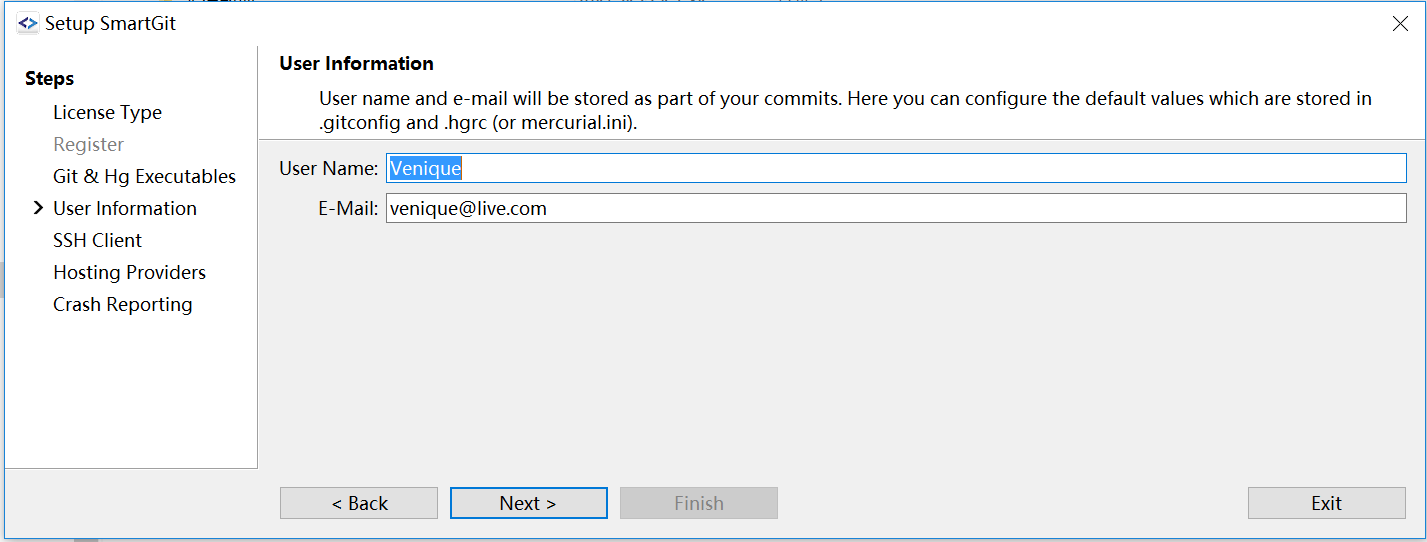
\includegraphics[width=0.8\textwidth]{user-name.PNG}
            \caption{填写任意用户名和邮箱,主要用于区分是谁提交的修改}
        \end{figure}        

        \begin{figure}[H]
            \centering
            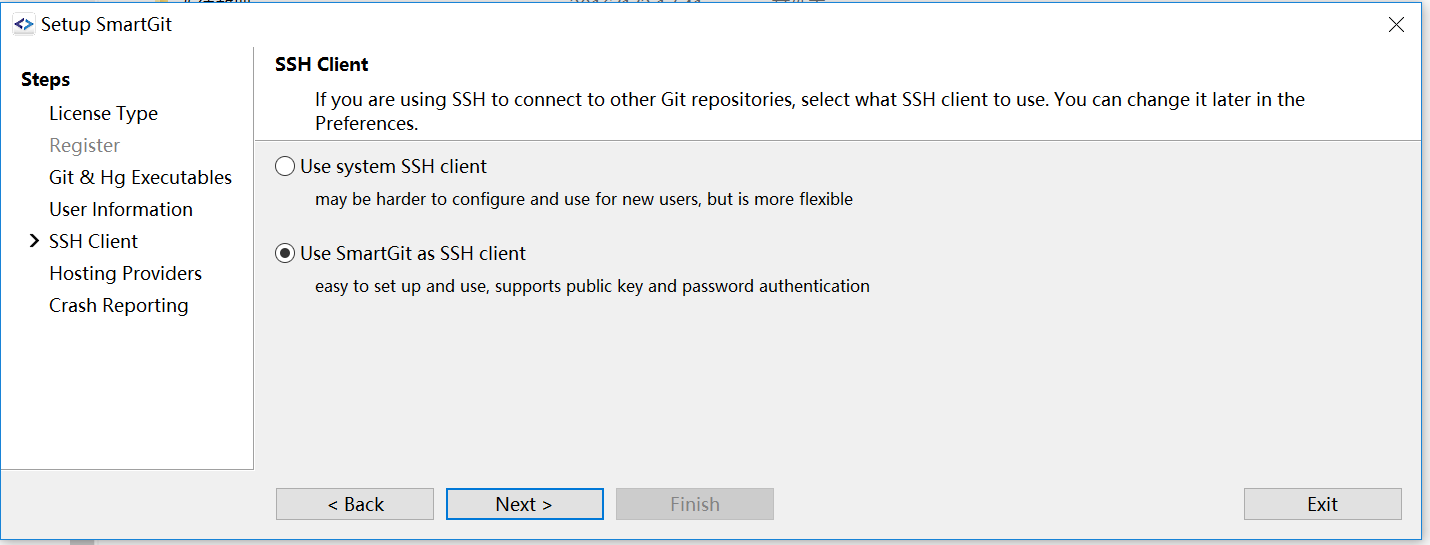
\includegraphics[width=0.8\textwidth]{ssh.PNG}
            \caption{使用SmartGit内置的ssh客户端}
        \end{figure}        

        \begin{figure}[H]
            \centering
            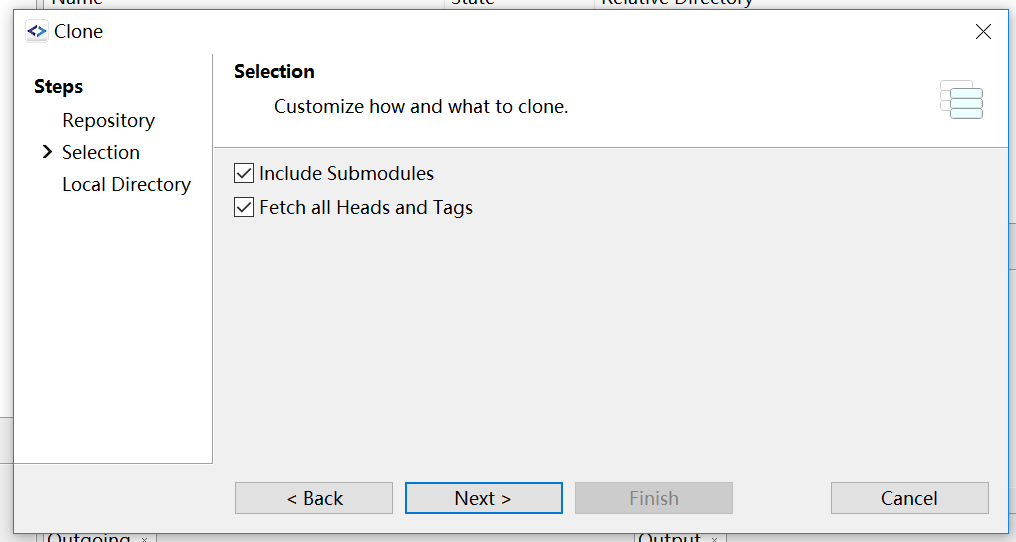
\includegraphics[width=0.8\textwidth]{finish.PNG}
            \caption{默认设置即可}
        \end{figure}        

        接下来就是选择同步到本地的那个地方了。自行解决即可。

        接下来介绍SmartGit的几个主要的功能。

    \newpage

    \section{SmartGit各功能简单介绍}
        Git是什么我就不介绍了,这里主要介绍几个比较常用到的功能:

        \begin{enumerate}[(1)]
            \item pull

                pull是用来从远程服务器上拉取当前最新的文件的。它可以自动将远程的文件和本地的文件合并(Merge),第一次运行merge的时候会进行初始化设置,如图\ref{fig:pull_setting}
                \begin{figure}[H]
                    \centering
                    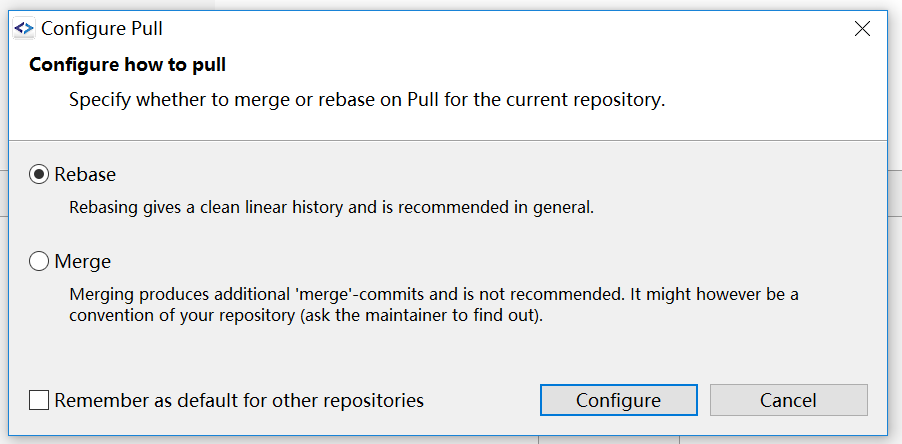
\includegraphics[width=0.8\textwidth]{pull.PNG}
                    \caption{设置pull的类型,选择推荐的默认类型就好了}
                    \label{fig:pull_setting}
                \end{figure}  

                在每次工作之前都建议进行一次pulll以保证本地版本和远程版本一致,如果在离线情况下可以不进行pull操作。

            \item Stage
                Stage是用来确认本地更改的,所有本地修改过的文件都会在Files窗口中显示,如图\ref{fig:stage}
                \begin{figure}[H]
                    \centering
                    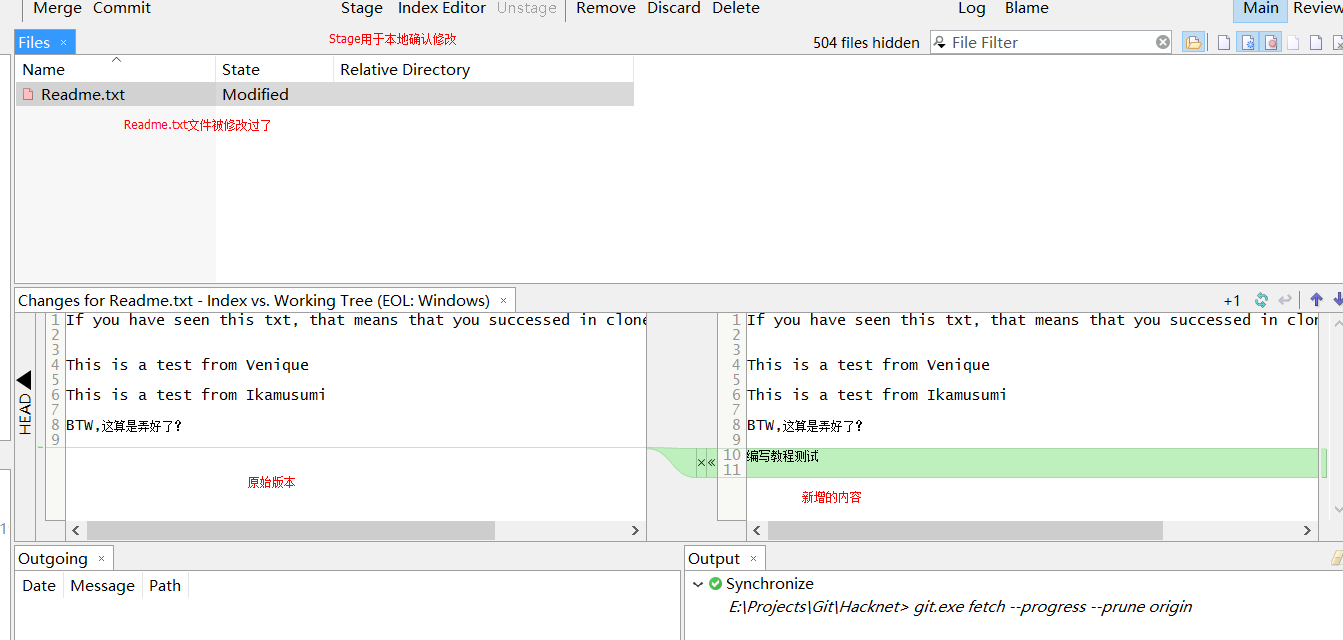
\includegraphics[width=0.8\textwidth]{Stage.png}
                    \caption{我在本地修改了Readme.txt,因而Files窗口自动显示出了Readme.txt,选中文件可以看到都做出了什么修改,点击Stage可以确认本次修改。之后状态从Modified变为Staged}
                    \label{fig:stage}
                \end{figure}

            \item \label{item:commit} Commit
                Commit是用来确认并登记本次所有Stage过的文件的,Commit必须提交相应的注释,具体介绍如图\ref{fig:commit}
                \begin{figure}[H]
                    \centering
                    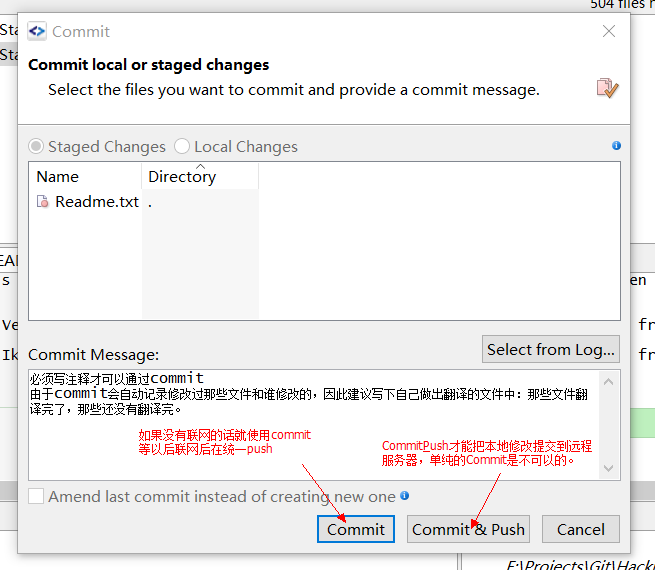
\includegraphics[width=0.8\textwidth]{commit.png}
                    \caption{一般在联网的情况下就直接commit\&push,如果离线的话就用commit暂存,注意最好按照要求编写注释}
                    \label{fig:commit}
                \end{figure}

            \item Push
                Push是用来把本地Commit过得修改提交到远程服务器的,如果步骤(\ref{item:commit})中进行的是commit\&push一般不需要使用Push,但是如果曾经commit过得话就需要在联网后\textbf{先进行pull},再进行push操作。如图:\ref{fig:push}
                \begin{figure}[H]
                    \centering
                    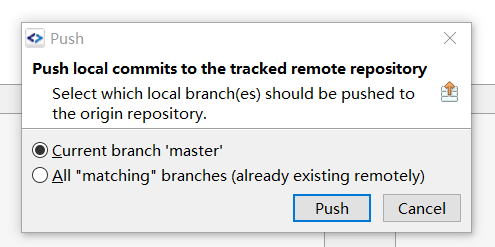
\includegraphics[width=0.8\textwidth]{push1.png}
                    \caption{按照默认的选项就行了}
                    \label{fig:push}
                \end{figure}

                在进行过push操作后,界面的Outgoing窗口的内容就会清空。



        \end{enumerate}

    \newpage

    \section{具体工作流程}
        设置完Git后,今后的工作流程就是:
        \begin{enumerate}[(1)]
            \item 进行一次pull操作,把远程服务器的最新版本与本地版本同步。
            \item 检查有没有合并冲突的,并手动解决合并冲突。
            \item 对本地文件进行翻译。
            \item 工作完成后检查并Stage所有修改过的文件。
            \item 最后commit\&push所有修改。
        \end{enumerate}

    \newpage

    \section{翻译格式要求:针对新加入群的}
        对于每一个文本的翻译(包括xml和txt文本)翻译格式要求如下:
        在文件头注明自己占用\textbf{每段英文下面的}第几行进行翻译\footnote{这主要是解决多人对同一个文件进行翻译的问题},如图\ref{fig:format}
        \begin{figure}[H]
            \centering
            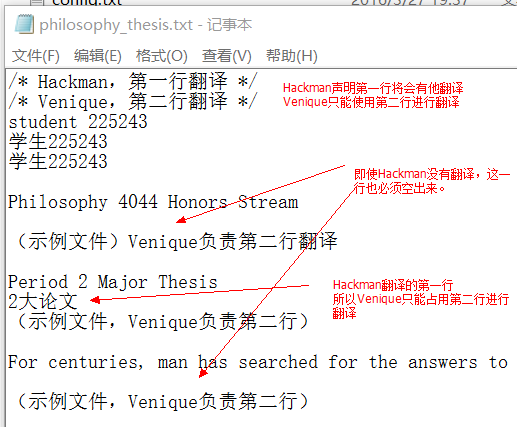
\includegraphics[width=0.8\textwidth]{format.png}
            \caption{翻译格式示例}
            \label{fig:format}
        \end{figure}

        \textbf{任何情况下,除了校审人员外,其他人不得修改他人的翻译!}目前校审人员有Venique,Sandman,Zhang,其他人如果觉得自己英语能力还行也可以找我报名

        校审格式如图\ref{fig:correct}
        \begin{figure}[!htbp]
            \centering
            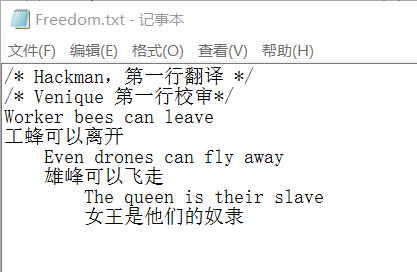
\includegraphics[width=0.8\textwidth]{correct.png}
            \caption{文件头按格式标注是谁进行的校审和对哪行校审,校审人员可以直接对他人翻译的文本进行修改}
            \label{fig:correct}
        \end{figure}

\end{document}

